\documentclass[11pt]{article}
\usepackage{latexsym}
\usepackage{amsmath}
\usepackage{amssymb}
\usepackage{amsthm}
\usepackage{epsfig}
\usepackage{bbm}

\usepackage[tight]{subfigure}

\usepackage{amsmath}

\DeclareMathOperator*{\minimize}{min}
\DeclareMathOperator*{\maximize}{max}

\usepackage{algorithm}
 %on linux you may need to run sudo apt-get install texlive-full to install algorithm.sys
\usepackage{algorithmic}

\usepackage{verbatim}

\newcommand{\handout}[5]{
  \noindent
  \begin{center}
  \framebox{
    \vbox{
      \hbox to 5.78in { {#1} \hfill #2 }
      \vspace{4mm}
      \hbox to 5.78in { {\Large \hfill #5  \hfill} }
      \vspace{2mm}
      \hbox to 5.78in { {\em #3 \hfill #4} }
    }
  }
  \end{center}
  \vspace*{4mm}
}

\newcommand{\lecture}[5]{\handout{#1}{#2}{#3}{#4}{#5}}
\newcommand{\collision}[0]{\mathrm{collision}}
\newcommand{\nocollision}[0]{\overline{\collision}}

\newcommand*{\QED}{\hfill\ensuremath{\square}}

\newtheorem{theorem}{Theorem}
\newtheorem{corollary}[theorem]{Corollary}
\newtheorem{lemma}[theorem]{Lemma}
\newtheorem{observation}[theorem]{Observation}
\newtheorem{proposition}[theorem]{Proposition}
\newtheorem{definition}[theorem]{Definition}
\newtheorem{claim}[theorem]{Claim}
\newtheorem{fact}[theorem]{Fact}
\newtheorem{assumption}[theorem]{Assumption}
\newtheorem{note}[theorem]{Note}

% 1-inch margins, from fullpage.sty by H.Partl, Version 2, Dec. 15, 1988.
\topmargin 0pt
\advance \topmargin by -\headheight
\advance \topmargin by -\headsep
\textheight 8.9in
\oddsidemargin 0pt
\evensidemargin \oddsidemargin
\marginparwidth 0.5in
\textwidth 6.5in

\parindent 0in
\parskip 1.5ex
%\renewcommand{\baselinestretch}{1.25}

\begin{document}

\lecture{Statistical Techniques in Robotics (16-831, S21)}{Lecture \#13
  (Wednesday, March 17)}{Lecturer: Kris Kitani}{Scribes: Yuda Song, Jinkun Cao}{MAB-Thompsons Sampling}

\section{Review}
In the last lecture, we covered two multi-armed bandits algorithm: Explore-Exploit and UCB. Both algorithms can achieve sublinear regret by using concentration inequalities during the analysis. Here we give a brief review of the two algorithms.
\subsection{Algorithms}
The pseudocodes for Explore-Exploit and UCB are shown in Alg.~\ref{algo:exp2} and Alg.~\ref{algo:UCB} respectively.
\begin{algorithm}[H]
\caption{Explore-Exploit}
\label{algo:exp2}
\begin{algorithmic}[1]
\REQUIRE $M$
\FOR{$k=1,\;\cdots,\;K$}
\FOR{$m=1,\;\cdots,\;M$}
\STATE $a = k$
\STATE $\text{Receive}(r)$
\STATE $\widehat{\mu}_k = \widehat{\mu}_k + \frac{r}{M}$
\ENDFOR
\ENDFOR
\FOR{$t=KM,\;\cdots,\;T$}
\STATE $a^{(t)} = \arg\max_{k}\widehat{\mu}_k'$
\ENDFOR
\end{algorithmic}
\end{algorithm}

\begin{algorithm}[H]
\caption{UCB}
\label{algo:UCB}
\begin{algorithmic}[1]
\REQUIRE $\delta, T$
\FOR{$t=1,\;\cdots,\;T$}
\IF{$t \leq k$} 
\STATE $k = t$
\ELSE
\STATE $k = \arg\max_{k'} \left( \widehat{\mu}_{k'} + \sqrt{\frac{\log(2T/\delta)}{2T^{(t-1)}_{k'}}} \right)$
\ENDIF
\STATE $\text{Receive}(r^{(t)})$
\STATE $T^{t}_k = T^{(t-1)}_k + 1$
\STATE $T^{t}_{k'} = T^{(t-1)}_{k'}\; \forall k' \in [K]\setminus \{k\}$
\STATE $\widehat{\mu}_k = \frac{1}{T_{k}^{(t)}}\left( T^{(t-1)}_k \widehat{\mu}_k + r^{(t)}_k \right)$
\ENDFOR
\end{algorithmic}
\end{algorithm}

\subsection{Regret Analysis}
Now we review the regret bound of the two algorithms.
\begin{theorem}
[Regret Bound for Explore-Exploit] The regret bound of Explore-Exploit is:
\[R = \widetilde{\mathcal{O}}(K^{1/3}T^{2/3}).\]
\end{theorem}
\begin{theorem}[Regret bound for UCB]
The regret bound for UCB is:
\[R = \mathcal{O}\left( 2\sqrt{\log(2T/\delta)\sqrt{KT}} \right) = \widetilde{\mathcal{O}}(\sqrt{KT}).\]
\end{theorem}

\section{Bayesian Stochastic Bandit}
In this lecture, we continue our setting of stochastic bandits (no adversary).  And we would mainly learn Thompson Sampling~\cite{thompson1933likelihood} method.

The overall idea is that we want to keep a parametric estimation of the reward distribution. Given a prior of the distribution of the parameter, we want to update the posterior of the parameter distribution by the likelihood of the reward we witness at each round. So let's first introduce some notations here:
\begin{itemize}
    \item $p(\theta)$: parameter prior
    \item $p(r|a,\theta)$: reward distribution (likelihood)
    \item $h^{(T)} = (a^{(t)}, r^{(t)})_{t=1}^T$: history of actions and rewards
    \item $p(\theta|h^{(t)})$: the posterior of the parameter
\end{itemize}
But why are we keeping on estimating the posterior distribution of the parameter $\theta$? Since we assume that each reward is drawn from a parametrized distribution, which is the likelihood function:
\[r \sim p(r|a,\theta),\]
then if true parameters of likelihood function are known, the problem becomes easy: we can simply select the arm that gives the highest expected reward:
\[a = \arg\max_{k} \mathbb{E}_{p(r|a_k, \theta^{\ast}_k)}[r | a_k, \theta^{\ast}_k].\]
So that is the overall idea of Thompson Sampling: 
\textbf{we maintain a running estimate of the prior distribution hyperparameter by observing the rewards. Then we
select the best arm by sampling from the estimated posterior distribution.} The form of the posterier is 
\[p(\theta | h^{(t)}) = p(\theta| a^{(1)}, r^{(1)}, \dots, a^{(t)}, r^{(t)}).\]
As the distribution is really hard to parameterize and compute, we would first make the Markov assumption over this to continue the process, which is:
\[p(r^{(t)}|\theta,a^{(t)}, a^{(t-1)}, \dots, a^{(1)}) = p(r^{(t)}|\theta,a^{(t)}).\]
Then using Bayes rule, we have:
\begin{align*}
    p(\theta | h^{(t)}) &= p(\theta| a^{(1)}, r^{(1)}, \dots, a^{(t)}, r^{(t)}) \\
    &= \frac{p(r^{(1)}, \dots, r^{(t)} | a^{(1)}, \dots, a^{(t)}, \theta) p(\theta | a^{(1)}, \dots, a^{(t)})}{ p(r^{(1)}, \dots, r^{(t)} | a^{(1)}, \dots, a^{(t)})} \\
    &= \frac{p(r^{(1)}, \dots, r^{(t)} | a^{(1)}, \dots, a^{(t)}, \theta) p(\theta)}{ p(r^{(1)}, \dots, r^{(t)} | a^{(1)}, \dots, a^{(t)})} \\
    &= \frac{\prod_{t} p(r^{(t)}| a^{(t)}, \theta) p(\theta) }{\prod_{t} p(r^{(t)}| a^{(t)})}\\
    &\propto \prod_{t} p(r^{(t)}| a^{(t)}, \theta) p(\theta).
\end{align*}

We note that in the formula, the form of $\theta$ can be very diverse. It can be a scalar, a tensor or even weights of a deep neural network. All depends on how the problem is formulated and the tools used to tackle the problem. Also note that we can get a recursive form of the posterior:
\[ p(\theta | h^{(t)}) = p(r^{(t)}| a^{(t)},\theta) p(\theta | h^{(t-1)}). \]
Then to get the best estimate of the parameter, we just need to find:
\begin{align*}
    \widehat{\theta} &= \arg\max_{\theta_k} p(\theta_k | h^{(t)})\\
    &= \arg\max_{\theta_k} p(r^{(t)}| a^{(t)},\theta_k) p(\theta_k | h^{(t-1)}).
\end{align*}
Note that line 2 of the previous equation suggests that we can perform the estimation incrementally.

\section{Conjugate Priors}
But how do we parameterize the likelihood, posterior and prior for efficient updates? Let's first write out the general form of the posterior:
\begin{align*}
    \underbrace{p(\theta | x)}_{\text{posterior}} \propto \underbrace{p(x|\theta)}_{\text{likelihood}} \underbrace{p(\theta)}_{\text{prior}}.
\end{align*}
We can see that it will be favorable if posterior and the prior have the same type of distributions. In this case, they are called conjugate distributions.\\
For example, the Gaussian distribution is the Conjugate prior of the Gaussian likelihood function. Another example we will show below is that the Beta distribution is the conjugate prior of the Bernoulli distribution.
\subsection{Bernoulli distribution}
The Bernoulli distribution is the discrete probability distribution of a random variable which takes the value 1 with probability $\theta$ and the value 0 with probability $1-\theta$. Denote $r = \{0,1\}$ as the random variable with a Bernoulli distribution parametrized by $\theta$, we have 
\[p(r|\theta) = \theta^r (1-\theta)^(1-r).\]
\begin{figure}[t]
    \centering
    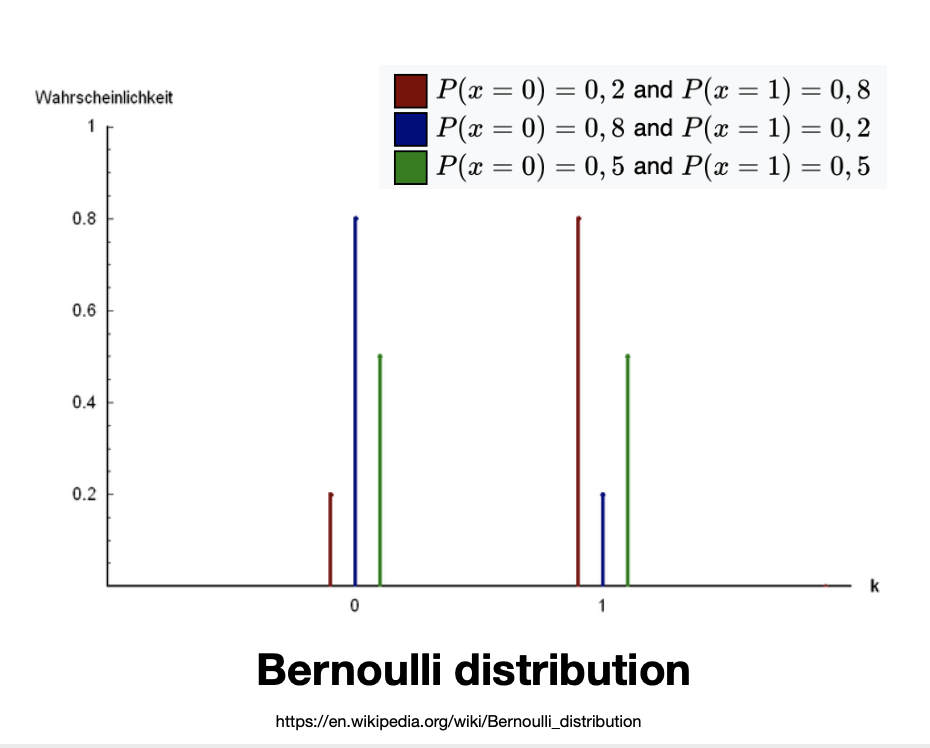
\includegraphics[width=0.5\textwidth]{figure/bernoulli.png}
    \caption{Bernoulli distribution}
    \label{fig:bernoulli}
\end{figure}

\subsection{Beta distribution}
Beta distribution is the probability distribution of the continuous random variable constrained in $[0,1]$. The probability distribution is defined by two positive shape parameters, $\alpha$ and $\beta$. Concretely, we write:
\[p(\theta) = \frac{\Gamma(\alpha + \beta)}{\Gamma(\alpha)\Gamma(\beta)} \theta^{\alpha-1}(1-\theta)^{\beta-1}, \]
where the Gamma function is defined as 
\[\Gamma(n) = (n-1)!.\]
\begin{figure}[H]
    \centering
    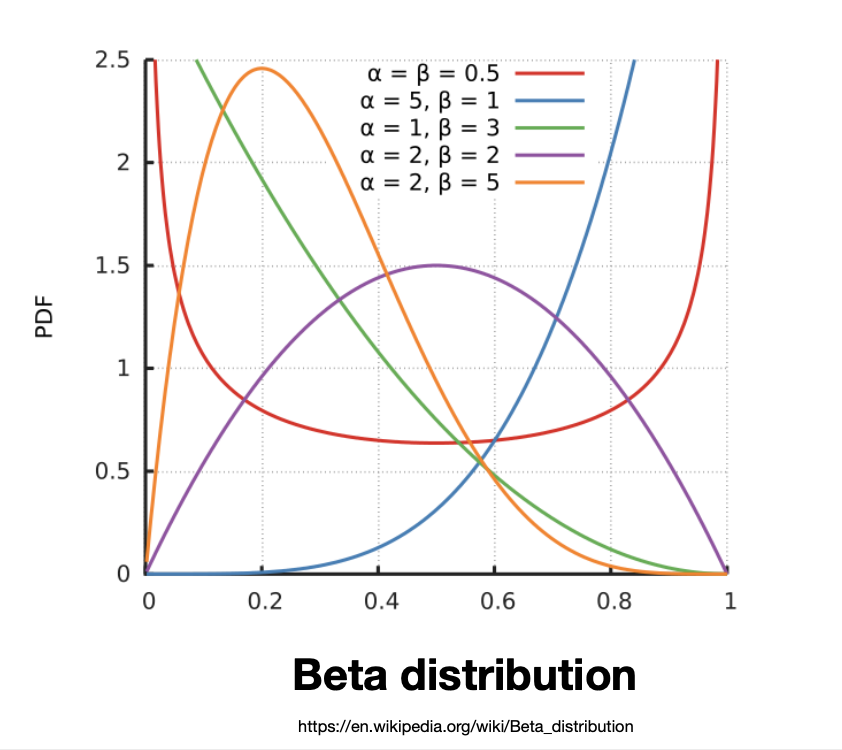
\includegraphics[width=0.5\textwidth]{lecture_13_B/figure/beta.png}
    \caption{Beta distribution}
    \label{fig:beta}
\end{figure}
\subsection{Beta-Bernoulli Bandit}
Now let's show that, in fact, the Beta distribution is the conjugate prior of the Bernoulli distribution. This will become very handy later when we want to estimate the posterior in the original problem.
\begin{proposition}
The Beta distribution is the conjugate prior of the Bernoulli distribution.
\end{proposition}
\begin{proof}
We have:
\begin{align*}
     \underbrace{p(\theta | r)}_{\text{posterior}} &\propto \underbrace{p(r|\theta)}_{\text{Bernoulli}} \underbrace{p(\theta)}_{\text{Beta}} \\
     &\propto \theta^r (1-\theta)^{1-r} \theta^{\alpha-1} (1-\theta)^{\beta-1}\\
     &\propto \theta^{r+\alpha-1} (1-\theta)^{1-r+\beta-1} \\
     &\propto \theta^{\alpha'-1} (1-\theta)^{\beta'-1},
\end{align*}
where $\alpha' = r+\alpha$ and $\beta = 1-r+\beta$. Thus we can see that the posterior is just another Beta distribution parametrized by $\alpha'$ and $\beta'$.
\end{proof}
Therefore, it is natural to form our bandit problem where we have a Beta prior on $\theta$ and the likelihood follows a Bernoulli distribution. Thus we can calculate the update rule for our estimations. Let's start with $t=1$, we have:
\begin{align*}
    p(\theta|r) &\propto p(r|\theta) p(\theta) \\
     &\propto \theta^r (1-\theta)^{1-r} \theta^{\alpha-1} (1-\theta)^{\beta-1}\\
     &\propto \theta^{r+\alpha-1} (1-\theta)^{1-r+\beta-1}\\
     &\propto \theta^{\alpha'-1} (1-\theta)^{\beta'-1}.
\end{align*}
And for time step $t$,

\begin{align*}
    p(\theta|h^{(t)}) &\propto p(r|\theta) p(\theta|h^{(t-1)}) \\
     &\propto \theta^r (1-\theta)^{1-r} \theta^{\alpha-1} (1-\theta)^{\beta-1}\\
     &\propto \theta^{r+\alpha-1} (1-\theta)^{1-r+\beta-1}\\
     &\propto \theta^{\alpha'-1} (1-\theta)^{\beta'-1}.
\end{align*}
Thus we see that, for each case, our update rule is just 
\[\alpha \xleftarrow{} \alpha + r\]
and 
\[\beta \xleftarrow{} \beta+1 - r.\]

\section{Thompson Sampling}
\subsection{Algorithm}
Now we are ready to introduce the algorithm. We covered three variants in the class, and we will show them in Alg.~\ref{algo:TS:batch}, Alg.~\ref{algo:TS:incremental} and Alg.~\ref{algo:TS:bb} respectively. Note the difference between the algorithms: in batch version, we update the posterior according the likelihood of all history data, while in the incremental version, we update according the the posterior of previous timestep and the likelihood of current timestep. The Bernoulli-Beta Thompson Sampling algorithm is just an instance of incremental version of Thompson Sampling in Bernoulli-Beta Bandits settings.
\begin{algorithm}[H]
\caption{Thompson Sampling (Batch Version)}
\label{algo:TS:batch}
\begin{algorithmic}[1]
\REQUIRE $\delta, T$
\FOR{$t=1,\;\cdots,\;T$}
\STATE $\theta_k \sim p(\theta_k|h_k)\; \forall k$
\STATE $a_{\widehat{k}}^{(t)} = \arg\max_{k} \mathbb{E}_{p(r|a_k, \theta_k)}[r]$
\STATE $\text{Receive}(r^{(t)})$
\STATE $h_{\widehat{k}} = h_{\widehat{k}} \bigcup (r^{(t)}, a_{\widehat{k}}^{(t)})$
\STATE $p(\theta_{\widehat{k}} | h_{\widehat{k}}) \propto p(h_{\widehat{k}}|\theta_{\widehat{k}}) p(\theta_{\widehat{k}} )$
\ENDFOR
\end{algorithmic}
\end{algorithm}

\begin{algorithm}[H]
\caption{Thompson Sampling (Incremental Version)}
\label{algo:TS:incremental}
\begin{algorithmic}[1]
\REQUIRE $\delta, T$
\FOR{$t=1,\;\cdots,\;T$}
\STATE $\theta_k \sim p(\theta_k|h_k)\; \forall k$
\STATE $a_{\widehat{k}}^{(t)} = \arg\max_{k} \mathbb{E}_{p(r|a_k, \theta_k)}[r]$
\STATE $\text{Receive}(r^{(t)})$
\STATE $p(\theta_{\widehat{k}} | h_{\widehat{k}}) \propto p(r^{(t)}|a^{(t)}_{\widehat{k}}, \theta_{\widehat{k}}) p(\theta_{\widehat{k}} | h_{\widehat{k}})$
\ENDFOR
\end{algorithmic}
\end{algorithm}

\begin{algorithm}[H]
\caption{Thompson Sampling (Bernoulli-Beta)}
\label{algo:TS:bb}
\begin{algorithmic}[1]
\REQUIRE $\delta, T$
\FOR{$t=1,\;\cdots,\;T$}
\STATE $\theta_k \sim p(\theta_k|h_k)\; \forall k$
\STATE $a_{\widehat{k}}^{(t)} = \arg\max_{k} \mathbb{E}_{p(r|a_k, \theta_k)}[r]$
\STATE $\text{Receive}(r^{(t)})$
\STATE $\alpha_{\widehat{k}} = \alpha_{\widehat{k}} + r^{(t)}$
\STATE $\beta_{\widehat{k}} = \beta_{\widehat{k}} +1- r^{(t)}$
\ENDFOR
\end{algorithmic}
\end{algorithm}

\subsection{Performance}
Not surprisingly, Thompson sampling is a no regret algorithm. Here we provide the regret bound:
\begin{theorem}[Regret of Thompson Sampling]
The regret of Thompson Sampling is
\[R(T) = O(\sqrt{KT\log(T)}) = \widetilde{O}(\sqrt{KT}).\]
\end{theorem}
On the other hand, the literature~\cite{chapelle2011empirical} shows that Thompson sampling actually enjoys excellent empirical performance, comparing with UCB:
\begin{figure}[H]
    \centering
    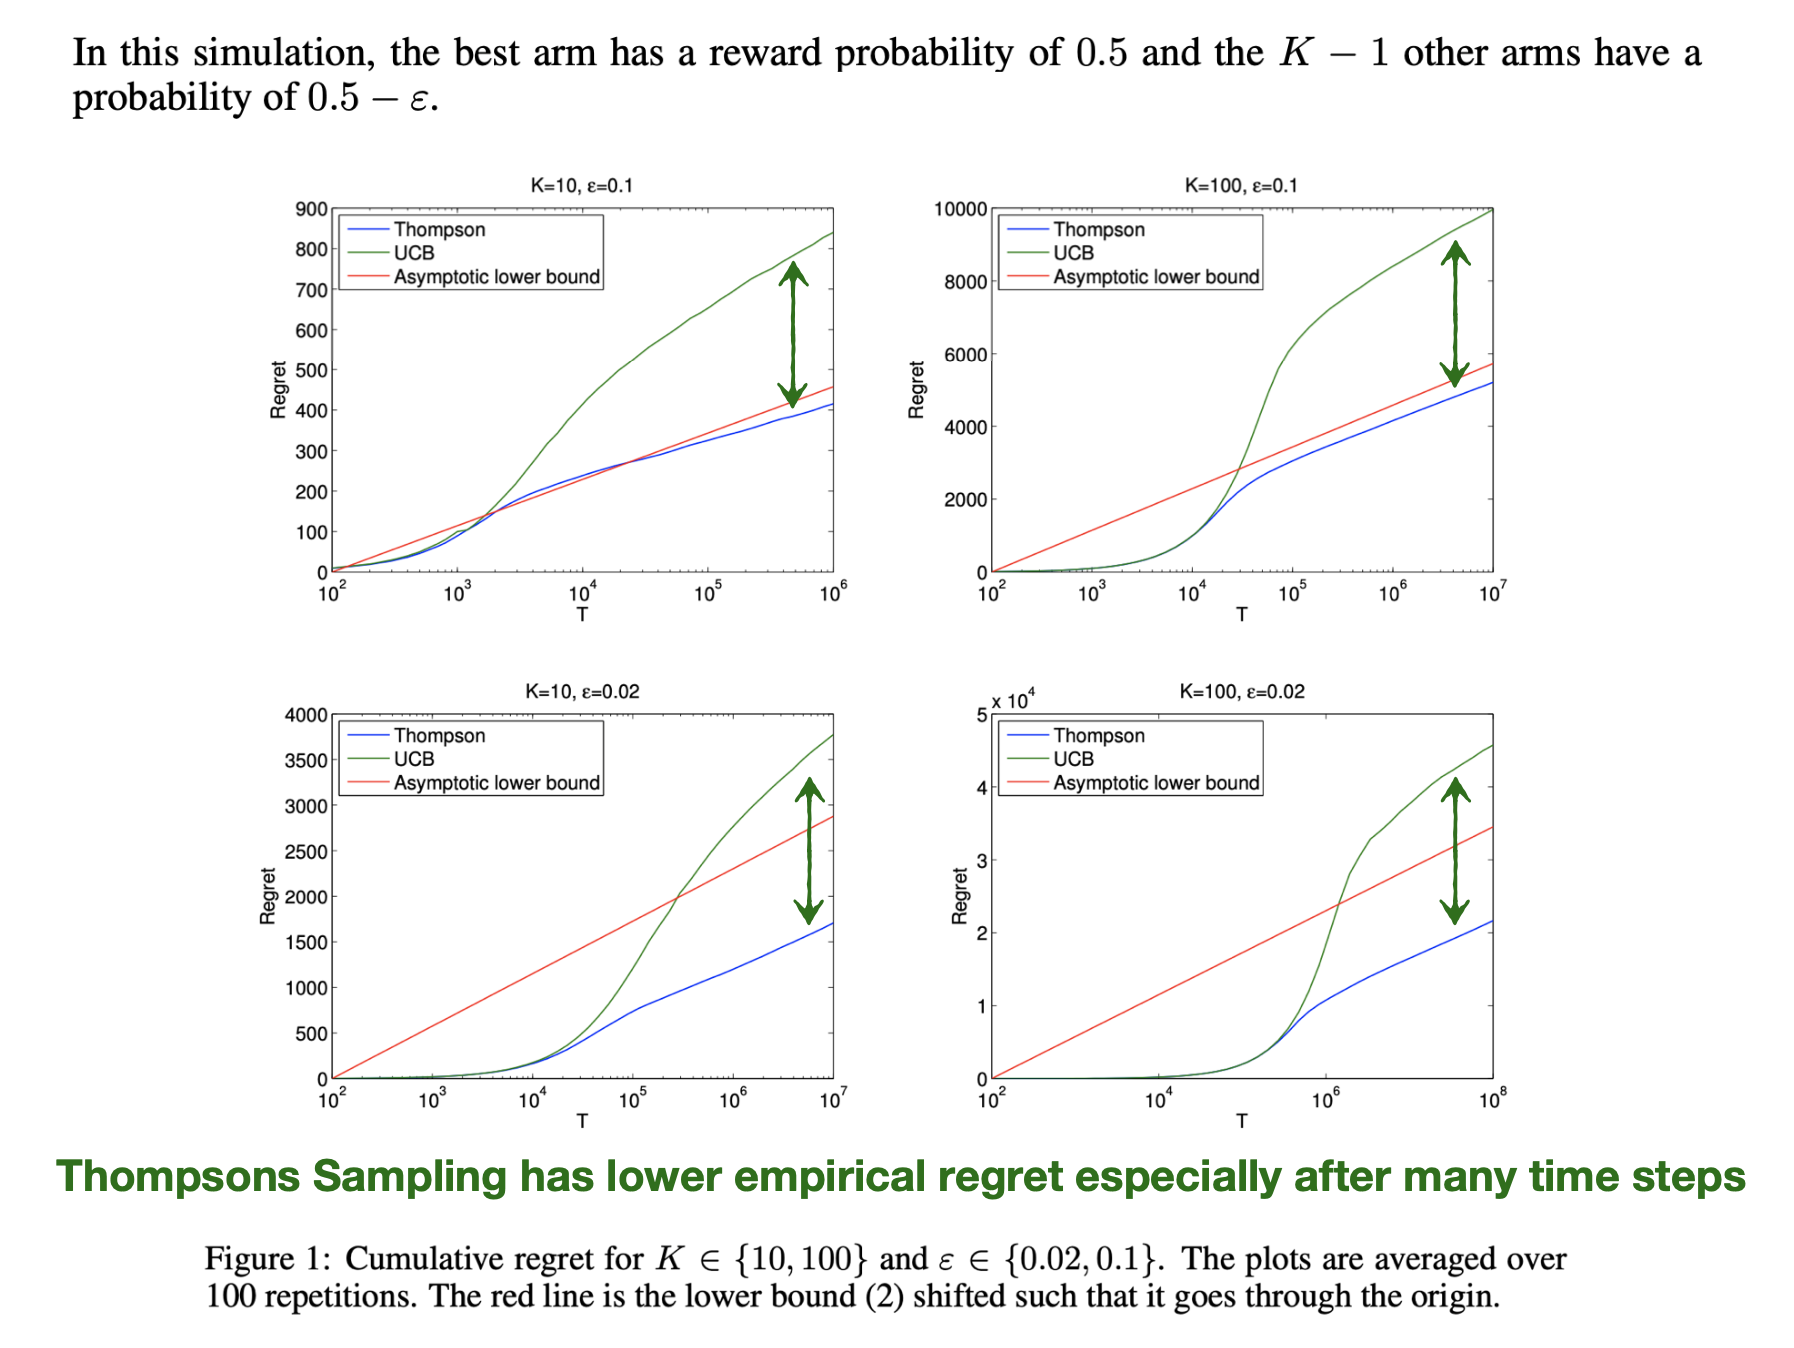
\includegraphics[width=1\textwidth]{figure/emp.png}
    \caption{Empirical performance of Thompson sampling.}
    \label{fig:beta}
\end{figure}

\section{Conclusion}
In this lecture, we studied the classic Thompson Sampling algorithm under the stochastic bandit environment. In such environment, we assume that the feedback from the environment is not contextual that it basically have a fixed underlying distribution to map the action to the reward. To find a good strategy maximizing reward from the environment, it is essential to solve an expectation maximum problem with a known parametric distribution of reward while that is what we just do not know in usual situations. So the problem comes to estimating the distribution of reward by historical observations. Then, the basic philosophy of Thompson Sampling comes: by maintaining a running estimation of the prior hyperparameter of rewards with historical observation, we select the *best* arm by sampling from the estimated posterior distribution.

Thompson Sampling is proven a non-regret algorithm, but the empirical experiments~\cite{chapelle2011empirical} shows that it actually enjoys performance gains when compared with UCB.

{
\bibliography{lec13refs}
\bibliographystyle{abbrv}
}

\newpage
\section{Appendix}
There are some truly wonderful materials to help us learn about about Thompson Sampling. For example, a Stanford tutorial~\footnote{https://web.stanford.edu/~bvr/pubs/TS\_Tutorial.pdf} covers more backgrounds, contents and extension following the problem and philosophy of Thomspon Sampling. Moreover, with the rise of deep learning, many researchers are looking into combining deep models with Thompson Sampling strategy. 

\subsection{More analysis of Thompson Sampling}

For the regret bound of Thompson Sampling, there is a paper~\cite{agrawal2013further} provides a new path to prove  the first near-optimal problem-independent bound of $O(\sqrt {NT\ln T})$ on the expected regret of this algorithm. This paper is pretty hardcore, but even more amazing to provide more advanced knowldege about Thompson Sampling. 

Besides, another wonder Stanford paper~\cite{russo2016information} provides an information-theoretic analysis of Thompson sampling that applies across a broad range of online optimization problems in which a decision-maker must learn from partial feedback. In many practical cases, the analysis provided in this work might be more useful than the generic or other forms of Thompson Sampling we learned during the class.

\subsection{Combining Thompson Sampling and Deep Learning}

Similar to the assumption of what we made during class, a previous work~\cite{riquelme2018deep} conducts an empirical comparison of performance in using approximate
Bayesian methods under a Thompson Sampling framework in reinforcement learning. They benchmark a series of related works over different contextual bandit problems in online settings. This would be an interesting literature to read if you have interest in the direction of reinforcement learning of posterior estimation under the Thompson Sampling framework to solve online problems.


There is another work combining Thompson Sampling with deep learning~\cite{zhang2020neural}. The authors propose a new algorithm, called Neural Thompson Sampling, which adapts deep neural networks for both exploration and exploitation. At the core of our algorithm is a novel posterior distribution of the reward, where its mean is the
neural network approximator, and its variance is built upon the neural tangent features of the corresponding neural network. They prove in the paper that, provided the underlying reward function is bounded, the proposed algorithm is guaranteed to achieve a cumulative regret of $O(T^{1/2})$,
which matches the regret of other contextual bandit algorithms in terms of total round number T.


There are actually much more interesting novel application or advanced analysis of Thompson Sampling, we just show some ones we found above to provide little inspiration of leveraging Thompson Sampling, the classic strategy developed decades ago, in more modern and newly born problems with more advanced tools we are familiar with today.
%This section provides any relevant background material that was not covered in the lectures, but was found to be useful for understanding the material. 
%For example, derivations, theory underlying techniques employed, etc. 

%Additionally, this section can summarizes applications or extensions of these techniques found in the literature. 

\end{document} % Done!


